\documentclass[12pt, a4paper]{article}
\usepackage[utf8]{inputenc}
\usepackage{amsmath}
\usepackage{amssymb}
\usepackage{natbib}
\usepackage{mathtools}
\usepackage{titling}
\usepackage[hidelinks]{hyperref}
\usepackage{booktabs}
\usepackage{float}
\usepackage{pbox}
\usepackage{adjustbox}
\usepackage{MnSymbol}
\usepackage{wasysym}
\usepackage{geometry}

\usepackage {tikz}
\usetikzlibrary{arrows}
\usetikzlibrary{shapes.misc, positioning, shapes.geometric}

\usepackage[font={it}, labelfont=bf]{caption}
\usepackage{graphicx}

%\usepackage{setspace}
%\doublespacing

\graphicspath{ {../images/} }

\author{Reid McIlroy-Young}
\title{An Novel RNN Approach to Classification of Complex Textual Scientific Metadata \\ \quad \\ \large MACS 30200 Final Paper}
\date{June 4, 2017}

\setcounter{tocdepth}{2}

\begin{document}
\pagenumbering{Roman}
\maketitle
\begin{abstract}
	\thispagestyle{plain}
	\textit{
		I introduce a new method for supervised classifying scientific metadata. This deep learning approach works with small and messy training data to provide high levels of accuracy. Using the method I analysis the introduction of new software tools to the statistics community.
	}
\end{abstract}		
\newpage
\tableofcontents
\newpage
\listoffigures
\newpage
\listoftables

\newpage
\setcounter{page}{1}
\pagenumbering{arabic}

\section{Introduction}

Currently most analysis of scientific publications is limited to those fields available in the database used by the researchers. Efforts to extend the fields usually rely on unsupervised clustering (e.g. \cite{Boyack2005}). These methods are useful and have greatly increase out understanding of how science works as a social phenomena. But, if we want to find paper with properties not given in the standard databases the usual solution is hand coding, which is either time consuming or expensive (usually both).

Recent developments in deep learning \citep{karpathy2015deep} have been highly successful at labelling/classifying very complex inputs, usually text or images. These techniques rely on large training datasets which are not available for biometric tasks and thus very little work has been done with scientific metadata. By relaxing the purity requirements of the training data we shows that sufficiently large training data can be generated and that it produces useful results.

The classification problem I am interested in is identifying \textit{papers introducing new software packages, tools or interfaces}. This aspect of the literature has not been previously analysed like this due to data limitations. Thus this method allows me to with high confidences give broad statistics about software usage in statistics that have never been calculated before.


\section{Literature Review}

Computer's have been a formal part of scientific work since the 18th Century \citep{grier2013computers}, but the modern day electromechanical machines developed by Turing \citep{turing1937computable} and many others \citep{abbate2012recoding}\citep{abbate2000inventing} are a much more recent innovation, of the last century \citep{bauer1972software}.  The introduction of these devices to communities around the world (both metaphorically and literally) has had major impacts on the culture \citep{lessig2007code}, technology\citep{abbate2000inventing} and rate of development \citep{bauer1972software}. Much work has been done to study these effects, but it has been primarily focused on either the macro cultural effects \citep{pfaffenberger1988social} or the economic/business usage \citep{landauer1995trouble}. 

By comparison the usage of computers by scientists has been overlooked by researchers \citep{sloanrep}. This oversight has many reasons, but one of the most significant is the lack of available data. The primary methods for large scale analysis of the culture or structure of scientific work involve bibliometric techniques \citep{de2009bibliometrics} using large standard datasets\citep[e.g.][]{Boyack2005, borner2010atlas, borner2015atlas, sugimoto2013global, shi2015weaving, evans_meta, skupin2013visualizing}. These dataset are generally lacking information about the computational aspects of the work, e.g. the  Clarivate Analytics Web of Science (WOS) does not have any such field \citep{mkdocs} and as such research into this dimension is difficult. Recent developments in natural language processing (NLP) have shown that complex concepts can be extracted reliably from text for a wide variety of tasks \citep{evans2016machine}, with some very similar to that done here \citep{foster2015tradition}.

\subsection{Information Extraction}

To extract the information about software usage from the available data requires complex NLP techniques and the best methodologies change quickly\citep{evans2016machine}. As we are primarily concerned with the classification of meta-data for a record relating it to a new software tool or not, in theory there are a large number of available techniques, as this is a simple binary classification problem \citep{james2013introduction}\citep{jurafsky2000speech}\citep{murphy2012machine}. We have considered most of the available techniques:

\begin{itemize}
\item Classified based on a simple regular grammar, e.g. regex
\item Word collocation frequencies \citep{manning1999foundations}
\item Term frequency–inverse document frequency vectors with an SVM or other classifier \citep{collobert2011natural}
\item Word2Vec vectors with an SVM or other classifier\citep{mikolov2013distributed}\citep{collobert2011natural}
\end{itemize}

The the current state of the art for natural language processing is the usage of deep neural networks for information extraction requiring more than simple word level similarities\citep{manning-EtAl}. As this is the state of the art there is no simple set of rules to follow, but there are some guidelines \citep{Goodfellow-et-al-2016}. These have lead us to the use of a recurrent neural network (RNN) \citep{mikolov2010recurrent} for the classification, although the exact specifics have been determined with cross-validation techniques \citep{james2013introduction}. The main features to consider are the type of regularization \citep{Goodfellow-et-al-2016}, what representation of words to use (most likely Word2Vec \citep{mikolov2013distributed}), what non-textual data will be included as there are in the WOS data set over 60 possible fields for each record \citep{mkdocs} and what values the hyperparameters take\citep{Goodfellow-et-al-2016}. This tuning is highly specific to the data, framework (in this case PyTorch \citep{pytorch} with NVIDIA's cuDNN \citep{chetlur2014cudnn}) and are described in further sections.

\subsection{Data Analysis}

Once the records with new software tools have been identified, we can use the existing theory of bibliometrics to look at the network structure. The literature standard approaches are to look at the structure of these nodes in the citation and authorship graphs \citep{de2002pattern}\citep{lariviere2006canadian}\citep{borgatti2009network}. This can be a computationally intensive task but tools exists that make it more practical \citep{mclevey2017introducing} so once the records have been labelled the analysis techniques are no longer novel.

The literature is silent on basic features of scientific software usage, and even when limited to only new releases there is no existing data. Thus simple measures such as per domain counts/frequencies and basic graph measurements such as the centrality will be new contributions. 

The other main question of what causes tools to be successful, has not been answered for scientists. There has been some work in the business domain \citep{xin2008software}\citep{hsu2009computer}. The adoption of new tools by businesses is theorized to follow a sigmoid pattern, with successful new entrants having three stages of usage: First they are used by early adopters and have small market penetration. Then they reach a "take off point" and the large majority of users will adopter their tools. Finally there will be slow growth in adoption again as only the laggards are left as new users \citep{xin2008software}. This is based on adopters having a Gaussian distributed chance of adopting the tool and notably this diffusion model does not require that the software have any costs for the users and allows for network effects, thus this signature is considered in our modelling.

There also has been work done examined open source projects \citep{mockus2002two} which agrees with the theory \citep{raymond1999cathedral} of open source that success is derived from openness and collaboration. This would predict that successful tools would come from highly connected groups who are working successfully with the community. This may show up as high connectedness in the co-authorship network correlating with success.

What leads to success has also be been studied in the context of ideas in the scientific literature \citep{acharya2004ideas} \citep{johntalk} or of individuals\citep{sinatra2016quantifying}. In both cases the main measure of success is the cumulative count of citations, which we can also examine on a per paper and a per author basis. We can look for the predictors of success for a new software tool by examining its citations over time and us this as our measurement for the signature. Notably \cite{sinatra2016quantifying} show a that success very unpredictable and can happen years after the paper is published. If the software records have patterns matching this model then the diffusion model may not be a good fit.

\section{Data}

The source of data used for this analysis is the  Web of Science (WOS) database hosted by Knowledge Lab. It has metadata on almost all scientific publications from 1960 to 2015, with new records being more complete. Each publication can be linked to one or more other tables each which contain other metadata than the main table, the number of entries for each table I am concerned with are shown in Table \ref{wos} and the complete database schema in Figure \ref{schema}. Access to the database is controlled by Knowledge Lab so they would need to be contacted to access it, once access rights are obtain the database is found at \href{wos2.cvirc91pe37a.us-east-1.rds.amazonaws.com}{wos2.cvirc91pe37a.us-east-1.rds.amazonaws.com} and the documentation at \href{http://docs.cloudkotta.org/dataguide/wos.html}{http://docs.cloudkotta.org/dataguide/wos.html}.

The data for WOS were collected by Thompson Reuters until 2016, when it was given to  Clarivate Analytics who now maintain it. The contemporary publications are collected from the publishers directly while older and more obscure publications are obtained from scanned copies digitalized with OCR, which is one of the factors that leads to newer publications having much higher quality data.

\begin{table} [!ht]
	\centering
	\begin{tabular}{lr}
		\toprule
		Table & Number of Entries\\
		\midrule
		publications & 57136685\\
		abstracts &	26093439\\
		publishers & 50668193\\
		keywords &	78155603\\
		references &	1085738245\\
		\bottomrule
	\end{tabular}
	\caption{Web of Science database number of entries per table}\label{wos}
\end{table}

\begin{figure}[H]
	\centering
	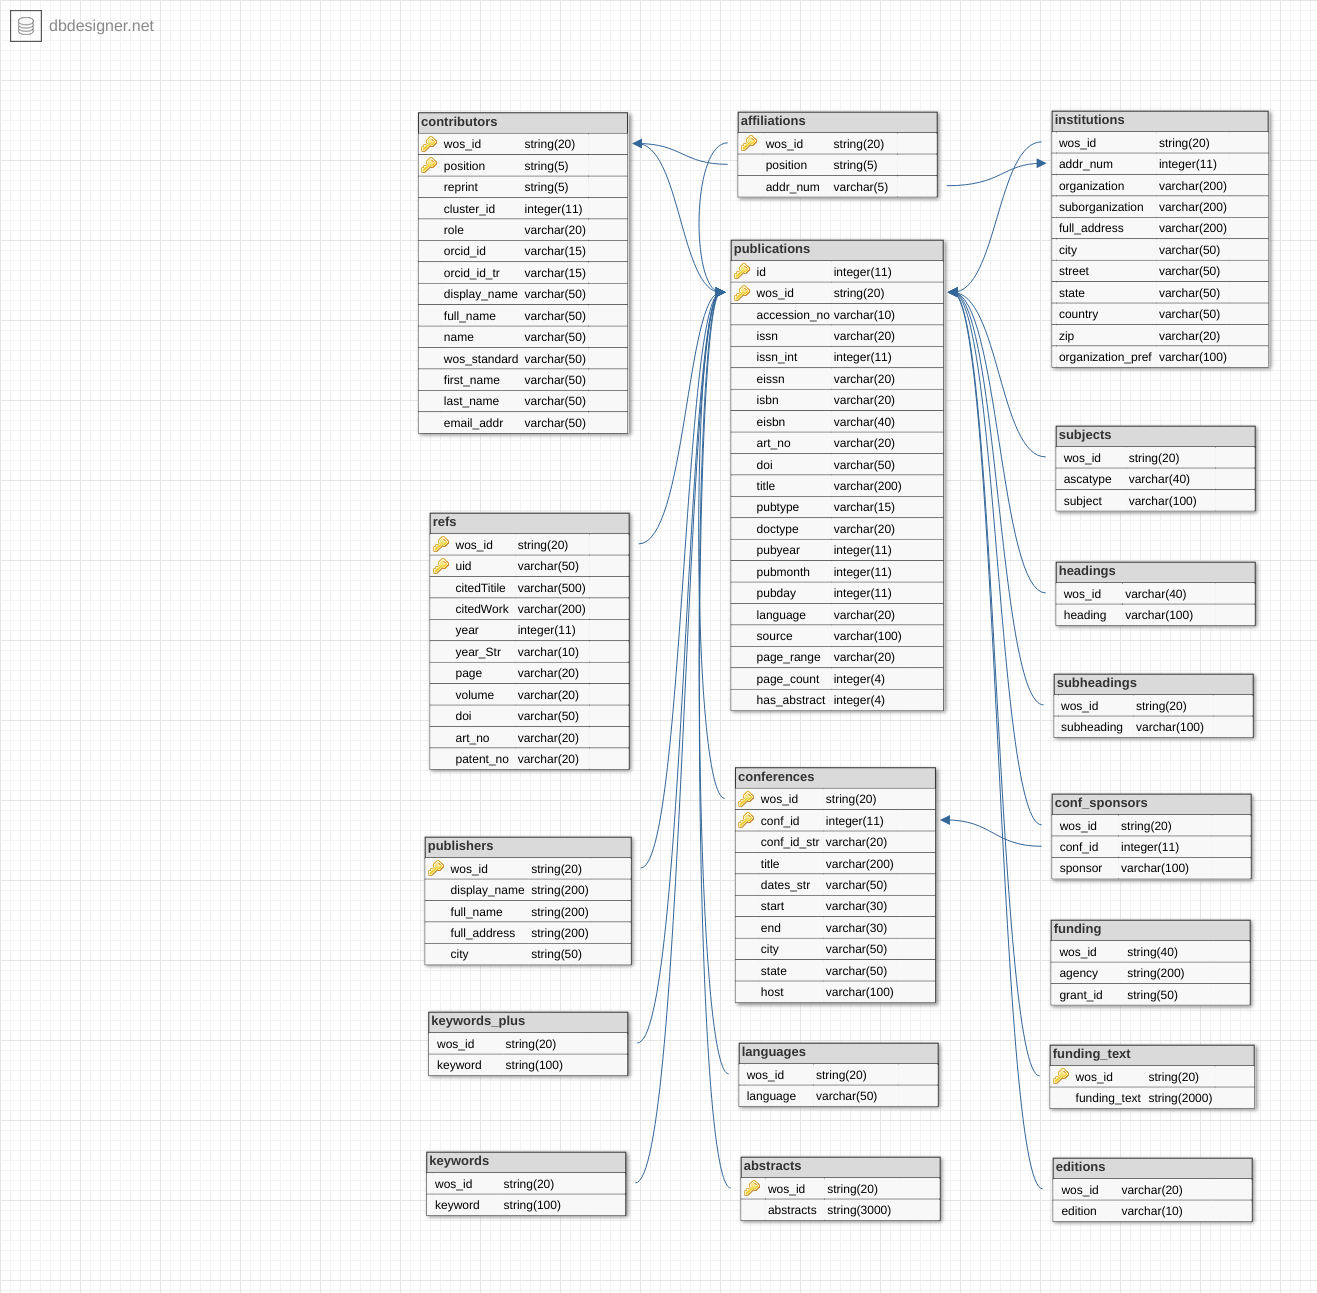
\includegraphics[width=\textwidth]{wos2_schema}
	\caption{Knowledge Lab WOS database schema}\label{schema}
\end{figure}
\newpage
For this analysis I limited my data to those journals from the top 123 statistics publications between 2005 and 2016, giving me a total of 78 971 articles (publications). From these I derived a training set of classified (training) and unclassified publications. To do this I found journals that almost entirely publish new scientific software, thus all articles from these can be classified as containing new software, i.e. as positive. There are also some that contain virtually none, all of their publications can then be classified as negative.  The classified journals are given in Table \ref{journals}, note they are all top statistics journals from the data set.

\begin{table}[H]
	\centering
	\begin{adjustbox}{center}
		\begin{tabular}{lccc}
			\toprule
			Journal & Classification & Total Citations & Impact Factor\\
			\midrule
			R JOURNAL & Mostly Software & 271 & 1.045\\
			STATA JOURNAL&Mostly Software&2636&1.292\\
			\pbox{20cm}{JOURNAL OF\\STATISTICAL SOFTWARE}&Mostly Software &6868&2.379\\
			&&&\\
			ECONOMETRICA&Little Software&24957&4.053\\
			TECHNOMETRICS&Little Software&6062&1.435\\
			\pbox{20cm}{STATISTICAL METHODS IN\\ MEDICAL RESEARCH}& Little Software &2703&4.634\\
			&&&\\
			\pbox{20cm}{JOURNAL OF THE ROYAL\\STATISTICAL SOCIETY SERIES\\B-STATISTICAL METHODOLOGY} &Little Software&2 360 &1.702\\
			&&&\\
			\pbox{20cm}{BRITISH JOURNAL OF MATHEMATICAL \&\\ STATISTICAL PSYCHOLOGY}&Little Software&1 278 &3.698\\
			&&&\\
			\pbox{20cm}{ANNUAL REVIEW OF STATISTICS\\ AND ITS APPLICATION}&Little Software&74 & 3.045\\
			&&&\\
			ANNALS OF STATISTICS&Little Software&15 680 &2.780\\
			\pbox{20cm}{STOCHASTIC ENVIRONMENTAL \\RESEARCH AND RISK ASSESSMENT}&Little Software&2 297 &2.237\\
			\bottomrule
		\end{tabular}
	\end{adjustbox}
	\caption{Classified journals with 2015 citations and impact factors}\label{journals}
\end{table}

When combined the I have a training set of 1251 positive and 4362 negative examples. This is not a large data set nor is it pure since some articles from the positive set are in fact negative, one example\citep{wickham2014tidy} is shown Figure \ref{badPos}. As there is no pre-existing known set of clean papers I cannot give an exact count of the incorrectly identified papers, but as I will discuss later the model is capable of identifying them despite their presence in the training set. The paper used here is one of the one identified by the fully trained model as being not software.

\begin{figure}[H]
	\begin{tabular}{ll}
		\toprule
		Field & Value\\
		\midrule
		ID & WOS:000341806800001 \\
		Source & JOURNAL OF STATISTICAL SOFTWARE \\
		Year of Publications & 2014 \\
		Title & Tidy Data \\
		Abstract & A huge amount of effort is spent cleaning data to get it ready for\\
		&analysis, but there has been little research on how to make data\\
		&cleaning as easy and effective as possible. This paper tackles a\\
		&small, but important, component of data cleaning: data tidying. Tidy\\
		&datasets are easy to manipulate, model and visualize, and have a\\
		&specific structure: each variable is a column, each observation is a\\
		&row, and each type of observational unit is a table. This framework\\
		&makes it easy to tidy messy datasets because only a small set of\\
		&tools are needed to deal with a wide range of un-tidy datasets. This\\
		&structure also makes it easier to develop tidy tools for data\\
		&analysis, tools that both input and output tidy datasets. The\\
		&advantages of a consistent data structure and matching tools are\\
		&demonstrated with a case study free from mundane data manipulation\\
		&chores. \\
		Citation & \cite{wickham2014tidy}\\
		\bottomrule
	\end{tabular}
	\caption{An example of a false positive in the training set}\label{badPos}
\end{figure}

\section{Methods}

The classifier works as a series of operations on the two input strings (the title and abstract). The first step is tokenizing which is done with the Python NLTK package \citep{Loper:2002:NNL:1118108.1118117}, this tokenizer is not perfect but it is deterministic and lossless which are both more important for this task. The tokens of interest are words and punctuation this string of tokens is then normalized to lower case and converted to Word2Vec \citep{mikolov2013efficient} word embedding vectors with gensim \citep{rehurek_lrec}. The embeddings are from a model trained on the entire corpus of abstracts and titles using  hierarchical softmax, with a window size of 5, as that is better with low frequency words\citep{mikolov2013efficient} than the alternative negative sampling \citep{mikolov2013distributed}. NLTK's sentence tokenizer was used along with its word tokenizer to generate the training sequences for the embedding, with titles treated as single sentences. The word embeddings primarily serve as a way of converting words into a vector space so the small sample size is not an issue. The output vectors are 200-dimensional and are defined for all tokens in the dataset, thanks to the deterministic parsing, for a total of 13 4420 tokens.

Once converted the title and abstract both become variable length sequences of 200-dimensional vectors these are then given to separate bidirectional \citep{graves2013hybrid} Long Short Term Memory (LSTM) layers ($h^1$ and $g^1$) \citep{Hochreiter:1997:LSM:1246443.1246450}, the LSTM implementation used is NVIDIA's cuDNN \citep{chetlur2014cudnn}. These layers each have 256 nodes which then feed to a second set of layer 256 node layers ($h^2$ and $g^2$) whose final activations are then combined to produce one 512-dimensional output, this forms the Recurrent Neural Network (RNN) for each of the inputs. The recurrent and LSTM connections are limited to within a layer and do not add to the outputs directly. Finally, outputs from the RNN layers are then combined are then fed into a single fully connected layer ($u$) that converts the two 512-dimensional outputs into a single 2-dimensional vector giving the log probabilities for each class ($\hat{y}$).

Figure \ref{rnn} shows a partially unrolled graph of the complete systems, and Table \ref{lt} gives the dimensions. The layers the circular nodes in the figure were all learned via backpropagation. Backpropagation weights updating was done with stochastic gradient descent using and an Adaptive Moment Estimation (ADAM) optimizer \citep{kingma2014adam}. Due to limitation of the RNN framework a mini-batch size of 1 was the only size available, i.e. after each training sample the weights were updated. For loss the cross entropy was used against a one-hot vector giving the true value, i.e. $[0, 1]^T$ or $[1, 0]^T$.

A $10\%$ random sample of the classified data was taken and used as a validation set with the rest left for training. Since sampling from the training data uniformly has only about a one in five chance of finding a positive example the model would find the local minima of responding negative to all samples. To solve this the positive samples were added to the sample pool twice giving about a one in three chance of being encountered. Then the training was divided into epochs of 500 exposures, after each epoch the testing error and testing loss was computed, these were then used to pick the final model's number of epochs, as discussed in the next section. 

\begin{table}[H]
	\centering
	\begin{adjustbox}{center}
	\begin{tabular}{|l|c|c|}
		\toprule
		Layer & Description&Operation\\
		\midrule
		Title & Raw title & $string$\\
		Abstract & Raw abstract & $string$\\
		Tokenizer & NLTK \texttt{word\_tokenize} & $string \rightarrow \{s_1 , s_2, \dots, s_n\}$\\
		Word2Vec & gensim \texttt{Word2Vec} $x_t$ & $s_t \rightarrow \mathbb{R}^{200}$ \\
		$h^1$ & forward 256-node $tanh$ activation and LSTM&$\mathbb{R}^{200} \rightarrow \mathbb{R}^{256}$\\
		$g^1$ & reverse 256-node $tanh$ activation and LSTM&$\mathbb{R}^{200} \rightarrow \mathbb{R}^{256}$\\
		$h^2$ & forward 256-node $tanh$ activation and LSTM&$\mathbb{R}^{256} \rightarrow \mathbb{R}^{256}$\\
		$h^2$ & reverse 256-node $tanh$ activation and LSTM&$\mathbb{R}^{256} \rightarrow \mathbb{R}^{256}$\\
		$\oplus$ & Concatenation of final activations &$\mathbb{R}^{256} , \mathbb{R}^{256} \rightarrow \mathbb{R}^{512}$\\
		$u$ & Fully connected linear layer  & $\mathbb{R}^{512}, \mathbb{R}^{512} \rightarrow \mathbb{R}^{2}$\\
		Loss & Cross Entropy Loss & $\mathbb{R}^{2}, \mathbb{R}^{2} \rightarrow \mathbb{R}^{1}$\\
		\bottomrule
	\end{tabular}
\end{adjustbox}
\caption{Specification of the model}\label{lt}
\end{table}


\begin{figure}[H]
\centering

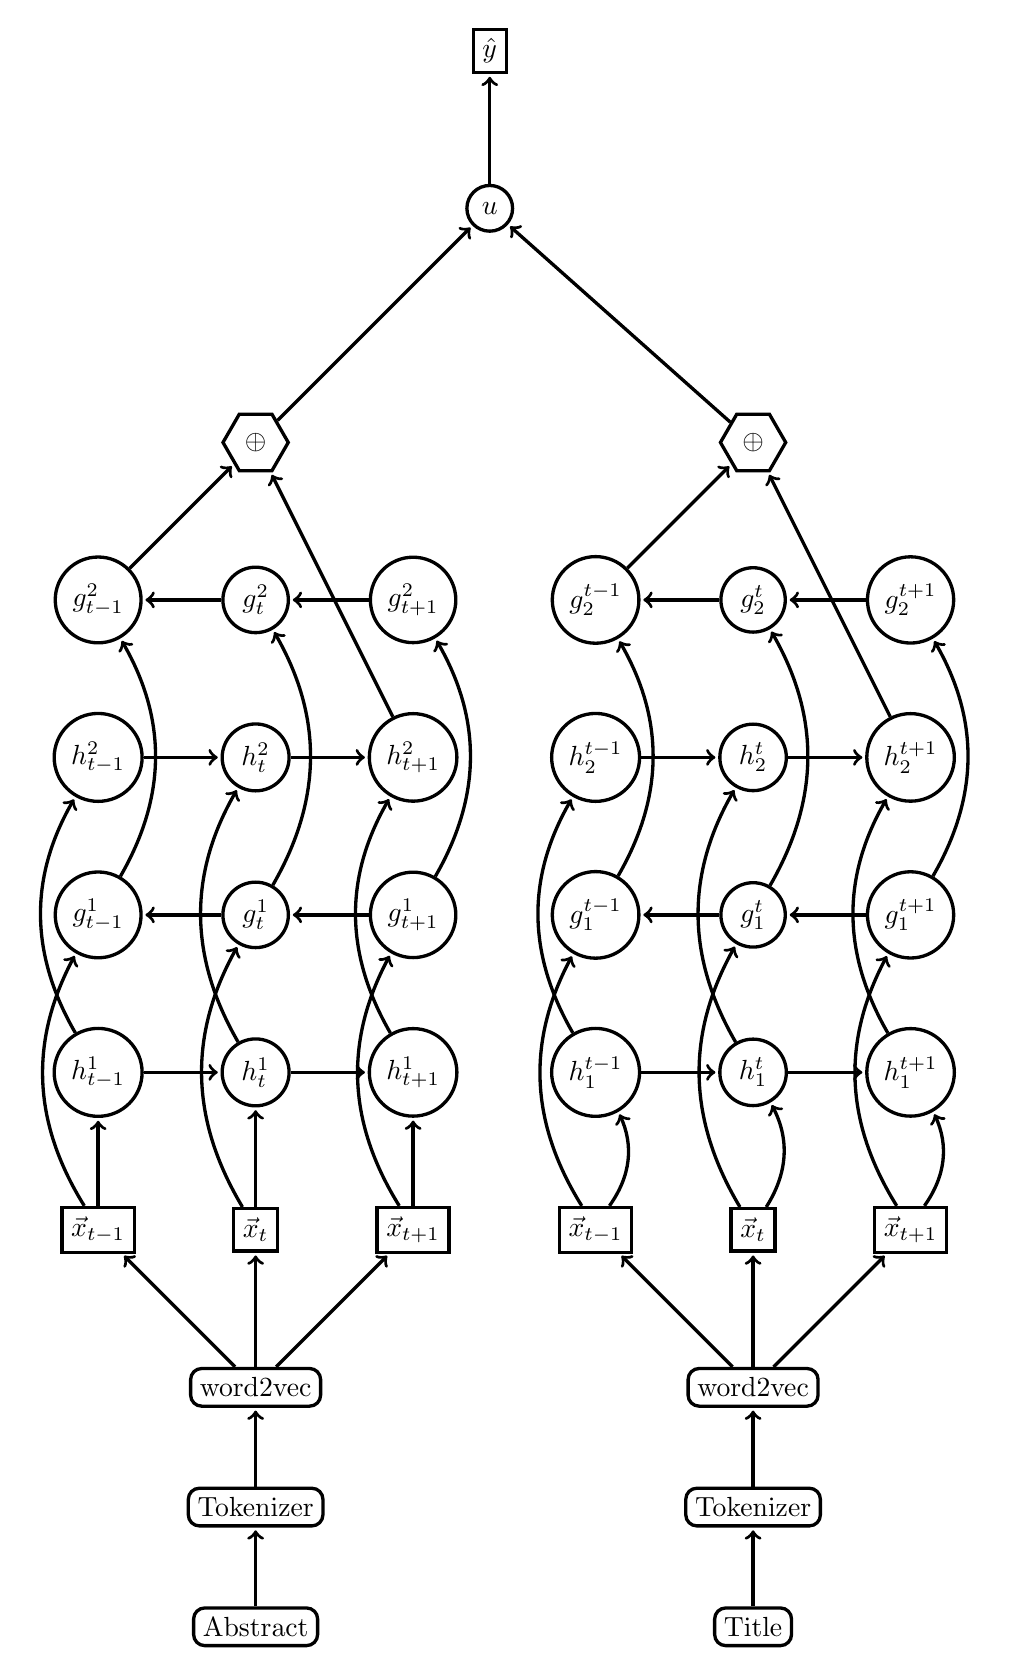
\begin{tikzpicture}[shorten >=1pt,auto,node distance=2cm, very thick]
\node[draw, rounded corners] (1) {Abstract};
\node[draw, rounded corners] (tokenizer) [above = 1cm of 1] {Tokenizer};
\node[draw, rounded corners] (2) [above = 1cm of tokenizer] {word2vec};
\node[draw] (3) [above of=2] {$\vec{x}_{t}$};
\node[draw] (4) [left of =3] {$\vec{x}_{t-1}$};
\node[draw] (5) [right of =3] {$\vec{x}_{t+1}$};

\node[draw, circle] (h1) [above of=3] {$h_t^1$};
\node[draw, circle] (h2) [above of=4] {$h_{t-1}^1$};
\node[draw, circle] (h3) [above of=5] {$h_{t+1}^1$};

\node[draw, circle] (g1) [above of=h1] {$g_t^1$};
\node[draw, circle] (g2) [above of=h2] {$g_{t-1}^1$};
\node[draw, circle] (g3) [above of=h3] {$g_{t+1}^1$};

\node[draw, circle] (h12) [above of=g1] {$h_t^2$};
\node[draw, circle] (h22) [above of=g2] {$h_{t-1}^2$};
\node[draw, circle] (h32) [above of=g3] {$h_{t+1}^2$};

\node[draw, circle] (g12) [above of=h12] {$g_t^2$};
\node[draw, circle] (g22) [above of=h22] {$g_{t-1}^2$};
\node[draw, circle] (g32) [above of=h32] {$g_{t+1}^2$};

\node[draw, regular polygon, regular polygon sides=6] (L) [above of=g12] {$\oplus$};

\node[draw, rounded corners] (1t) [right = 5cm of 1]{Title};
\node[draw, rounded corners] (tokenizert) [above = 1cm of 1t] {Tokenizer};
\node[draw, rounded corners] (2t) [above = 1cm of tokenizert] {word2vec};

\node[draw] (3t) [above of=2t] {$\vec{x}_{t}$};
\node[draw] (4t) [left of =3t] {$\vec{x}_{t-1}$};
\node[draw] (5t) [right of =3t] {$\vec{x}_{t+1}$};

\node[draw, circle] (h1t) [above of=3t] {$h^{ t}_1$};
\node[draw, circle] (h2t) [above of=4t] {$h^{ t-1}_1$};
\node[draw, circle] (h3t) [above of=5t] {$h^{t+1}_1$};

\node[draw, circle] (g1t) [above of=h1t] {$g^{t}_1$};
\node[draw, circle] (g2t) [above of=h2t] {$g^{t-1}_1$};
\node[draw, circle] (g3t) [above of=h3t] {$g^{t+1}_1$};

\node[draw, circle] (h1t2) [above of=g1t] {$h^{ t}_2$};
\node[draw, circle] (h2t2) [above of=g2t] {$h^{ t-1}_2$};
\node[draw, circle] (h3t2) [above of=g3t] {$h^{t+1}_2$};

\node[draw, circle] (g1t2) [above of=h1t2] {$g^{t}_2$};
\node[draw, circle] (g2t2) [above of=h2t2] {$g^{t-1}_2$};
\node[draw, circle] (g3t2) [above of=h3t2] {$g^{t+1}_2$};


\node[draw, regular polygon, regular polygon sides=6] (Lt) [above of=g1t2] {$\oplus$};
\node[draw, circle] (u) [above right = 3.5cm of L]{$u$};
\node[draw] (y) [above of = u]{$\hat{y}$};


\draw[->] (L) -- (u);
\draw[->] (Lt) -- (u);
\draw[->] (u) -- (y);

\draw[->] (1) -- (tokenizer);
\draw[->] (tokenizer) -- (2);
\draw[->] (2) -- (3);
\draw[->] (2) -- (4);
\draw[->] (2) -- (5);

\draw[->] (3) -- (h1);
\draw[->] (4) -- (h2);
\draw[->] (5) -- (h3);
\draw[->] (h2) -- (h1);
\draw[->] (h1) -- (h3);

\draw[->] (3)  edge[bend left] (g1);
\draw[->] (4) edge[bend left] (g2);
\draw[->] (5) edge[bend left] (g3);
\draw[->] (g1) -- (g2);
\draw[->] (g3) -- (g1);

\draw[->] (h1)  edge[bend left] (h12);
\draw[->] (h2) edge[bend left] (h22);
\draw[->] (h3) edge[bend left] (h32);
\draw[->] (h22) -- (h12);
\draw[->] (h12) -- (h32);

\draw[->] (g1)  edge[bend right] (g12);
\draw[->] (g2) edge[bend right] (g22);
\draw[->] (g3) edge[bend right] (g32);
\draw[->] (g12) -- (g22);
\draw[->] (g32) -- (g12);

\draw[->] (g22) -- (L);
\draw[->] (h32) -- (L);

\draw[->] (1t) -- (tokenizert);
\draw[->] (tokenizert) -- (2t);
\draw[->] (2t) -- (3t);
\draw[->] (2t) -- (4t);
\draw[->] (2t) -- (5t);

\draw[->] (3t) edge[bend right] (h1t);
\draw[->] (4t) edge[bend right] (h2t);
\draw[->] (5t) edge[bend right] (h3t);
\draw[->] (h2t) -- (h1t);
\draw[->] (h1t) -- (h3t);

\draw[->] (3t)  edge[bend left] (g1t);
\draw[->] (4t) edge[bend left] (g2t);
\draw[->] (5t) edge[bend left] (g3t);
\draw[->] (g1t) -- (g2t);
\draw[->] (g3t) -- (g1t);

\draw[->] (h1t)  edge[bend left] (h1t2);
\draw[->] (h2t) edge[bend left] (h2t2);
\draw[->] (h3t) edge[bend left] (h3t2);
\draw[->] (h2t2) -- (h1t2);
\draw[->] (h1t2) -- (h3t2);

\draw[->] (g1t)  edge[bend right] (g1t2);
\draw[->] (g2t) edge[bend right] (g2t2);
\draw[->] (g3t) edge[bend right] (g3t2);
\draw[->] (g1t2) -- (g2t2);
\draw[->] (g3t2) -- (g1t2);

\draw[->] (g2t2) -- (Lt);
\draw[->] (h3t2) -- (Lt);
\end{tikzpicture}
\caption[Unfolded Model Graph]{Simplified recursive bidirectional Recursive NN (RNN) layout, LSTM connections were removed for clarity. Circles are NN layers, rectangles with curved corners are the preprocessing, hexagons are combined outputs from the RNN layers, and final output and inputs are indicated with squared corners.}\label{rnn}
\end{figure}

\section{Results}

When evaluating the model the error rate can be broken into two components, the false positive rate and the false negative rate. Since the positives are sparse the false positive rate can become dominant if too high so it's minimization will have a much large impact than the maximization of the true positive rate (detection rate). Table \ref{epocst} shows the measured testing statics for 27 epochs (500 exposures of training data per epoch) of training for the data described in Table \ref{ttb}.

\begin{table}[H]
	\begin{tabular}{|l|ccc|}
		\toprule
		Set & Number of Negative & Number of Positive & Percentage Positive\\
		\midrule
		Training &3944 & 2216 & $36\%$\\
		Testing & 418 &143 & $25.5\%$ \\
		\bottomrule
	\end{tabular} 
\caption{Training-Testing breakdown}\label{ttb}
\end{table}
\begin{table}[H]
	\centering
	\begin{tabular}{|l|cccc|}
		\toprule
		Epoch & Loss & Error Rate & Detection Rate & False Positive Rate\\
		\midrule
		0 & 0.589 & 0.255 & 0.000 & 0.000\\ \hline
		1 & 0.363 & 0.185 & 1.000 & 0.249\\ \hline
		2 & 0.141 & 0.041 & 0.916 & 0.026\\ \hline
		3 & 0.172 & 0.043 & 0.937 & 0.036\\ \hline
		4 & 0.162 & 0.055 & 0.965 & 0.062\\ \hline
		5 & 0.129 & 0.032 & 0.944 & 0.024\\ \hline
		6 & 0.158 & 0.059 & 0.958 & 0.065\\ \hline
		7 & 0.123 & 0.030 & 0.937 & 0.019\\ \hline
		8 & 0.123 & 0.032 & 0.958 & 0.029\\ \hline
		9 & 0.110 & 0.034 & 0.923 & 0.019\\ \hline
		10 & 0.128 & 0.034 & 0.944 & 0.026\\ \hline
		11 & 0.113 & 0.029 & 0.944 & 0.019\\ \hline
		12 & 0.134 & 0.048 & 0.972 & 0.055\\ \hline
		13 & 0.177 & 0.032 & 0.895 & 0.007\\ \hline
		14 & 0.129 & 0.030 & 0.916 & 0.012\\ \hline
		15 & 0.131 & 0.043 & 0.881 & 0.017\\ \hline
		16 & 0.176 & 0.068 & 0.944 & 0.072\\ \hline
		17 & 0.178 & 0.057 & 0.951 & 0.060\\ \hline
		18 & 0.149 & 0.059 & 0.846 & 0.026\\ \hline
		19 & 0.177 & 0.061 & 0.811 & 0.017\\ \hline
		20 & 0.124 & 0.032 & 0.923 & 0.017\\ \hline
		21 & 0.126 & 0.025 & 0.951 & 0.017\\ \hline
		22 & 0.121 & 0.030 & 0.909 & 0.010\\ \hline
		23 & 0.115 & 0.027 & 0.937 & 0.014\\ \hline
		24 & 0.245 & 0.057 & 0.832 & 0.019\\ \hline
		25 & 0.233 & 0.062 & 0.790 & 0.012\\ \hline
		26 & 0.148 & 0.043 & 0.860 & 0.010\\ \hline
		27 & 0.127 & 0.034 & 0.916 & 0.017\\ \hline
	\end{tabular}
\caption{Testing results per epoch}\label{epocst}
\end{table}

As the table shows even after a six epochs the testing loss has nearly reached its minima this is fewer exposures than there are examples are in the training data so in theory the training data could be even smaller. As there was no major increase in testing statics to be gained from running training longer and to prevent over-fitting the model used for the rest of the analysis is that from epoch 7. This gives the final model the specification described in table \ref{t1}.

\begin{table}[H]
	\centering
	\begin{tabular}{l r}
		\toprule
		Epochs & 8  \\
		Batches per Epoch & 500\\
		Testing Loss &   0.093 \\
		Testing Error Rate & 0.023 \\
		Detection Rate & 0.955\\
		False Positive Rate& 0.017\\
		\bottomrule
	\end{tabular}
	\caption{Testing results for chosen model}\label{t1}
\end{table}

\subsection{Model Interpretation}

One issue with NN based models is there lack of interpretability, this makes declaring how our trained model works a near intractable problem, particularly for deep architecture like this one. To interpret or visualize the model there are few approaches, first we can embed the samples in a 2-dimensional space via some kind of dimension reduction. In fact since our outputs are 2-dimensional we can just use these. Sadly this does not work as the output variables are highly correlated as shown in figure \ref{pvn}. Also since the data are large texts there is no easy conversion for them into another visualization such as PCA or t-SNE.

\begin{figure}[H]
	\centering
	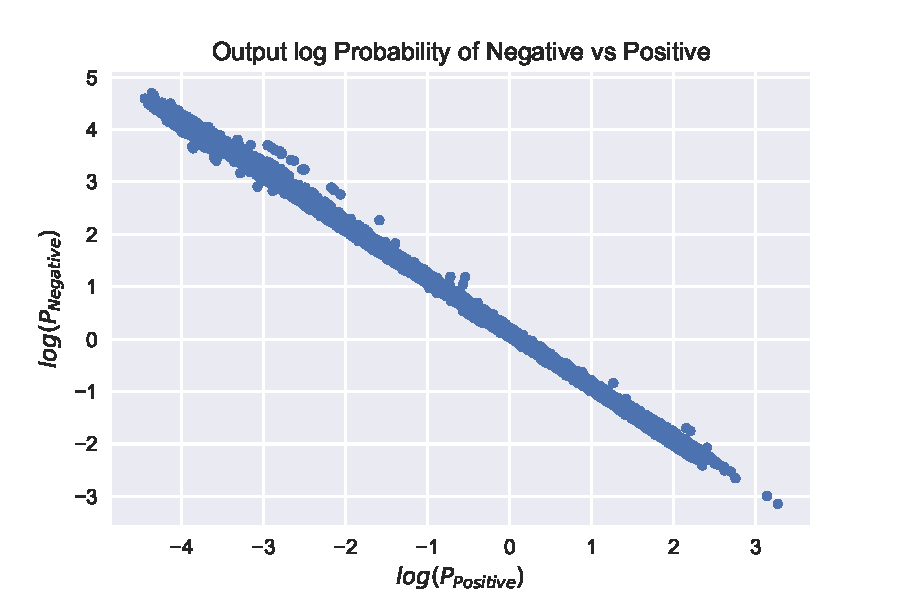
\includegraphics[width=\textwidth]{weight}
	\caption{Output for all samples from model}\label{pvn}
\end{figure}

What we can do is examine the activations of the NN layers for a single input. Unfortunately most of the work \citep{karpathy2015visualizing} in this focuses on the LSTM cells and other intermediate products which are not available to me dues to them being on the GPU inside NVIDIA's cuDNN implementation\citep{chetlur2014cudnn}. But was is available are the outputs from the RNN layers. Since all the RNN layer's outputs are the same dimension we can represent them as fixed width heatmaps with red being positive and blue negative and intensity showing magnitude. As an example we will be looking at two input articles a positive article Figure \ref{Pos} and a negative Figure \ref{Neg}, note only one is from the training set.

\begin{figure}[H]
	\begin{tabular}{ll}
		\toprule
		Field & Value\\
		\midrule
		ID & WOS:000365978900001 \\
		Source & JOURNAL OF STATISTICAL SOFTWARE \\
		Year of Publications & 2015 \\
		Title &  dawai: An R Package for Discriminant Analysis with Additional\\
		&Information \\
		Abstract &  The incorporation of additional information into discriminant rules\\
		&is receiving increasing attention as the rules including this\\
		&information perform better than the usual rules. In this paper we\\
		&introduce an R package called dawai, which provides the functions\\
		&that allow to define the rules that take into account this additional\\
		&information expressed in terms of restrictions on the means, to\\
		&classify the samples and to evaluate the accuracy of the results.\\
		&Moreover, in this paper we extend the results and definitions given\\
		&in previous papers (Fernandez, Rueda, and Salvador 2006, Conde,\\
		&Fernandez, Rueda, and Salvador 2012, Conde, Salvador, Rueda, and\\
		&Fernandez 2013) to the case of unequal co-variances among the\\
		&populations, and consequently define the corresponding restricted\\
		&quadratic discriminant rules. We also define estimators of the\\
		&accuracy of the rules for the general more than two populations case.\\
		&The wide range of applications of these procedures is illustrated\\
		&with two data sets from two different fields, i.e., biology and\\
		&pattern recognition. \\
		Citation &\cite{conde2015dawai}\\
		\bottomrule
	\end{tabular}
\caption{An example of a positive article}\label{Pos}
\end{figure}


\begin{figure}[H]
	\begin{tabular}{ll}
		\toprule
		Field & Value\\
		\midrule
		ID & WOS:000207446800001 \\
		Source & BAYESIAN ANALYSIS \\
		Year of Publications & 2006 \\
		Title & When Did Bayesian Inference Become "Bayesian"? \\
		Abstract &  While Bayes' theorem has a 250-year history, and the method of\\
		&inverse probability that flowed from it dominated statistical\\
		&thinking into the twentieth century, the adjective "Bayesian" was not\\
		&part of the statistical lexicon until relatively recently. This paper\\
		&provides an overview of key Bayesian developments, beginning with\\
		&Bayes' posthumously published 1763 paper and continuing up through\\
		&approximately 1970, including the period of time when "Bayesian"\\
		&emerged as the label of choice for those who advocated Bayesian\\
		&methods. \\
		Citation &\cite{fienberg2006did}\\
		\bottomrule
	\end{tabular}
	\caption{An example of a negative article}\label{Neg}
\end{figure}

You should be able to tell from reading the titles of each article if they introduce an new software package and so to it seems can the model. Figure \ref{title} shows the activations of the outer layers $g^2$ and $h^2$ at each word. The top figure is for the positive example, the middle for the negative and bottom a comparison of their final outputs. Since only the final outputs are used by the fully connected layer and thus learned with backpropagation they are much more significant than their predecessors. But the outputs of the penultimate and latter words can still be considered to be approximations of the final outputs since the RNN does not know if a word is the last.

By making this reasonable assumption we can further infer that the outputs are being updated as the RNN moves through the text, note the RNN reads it both forward and reverse once. Thus we can interpret each words activations as a description of the text up to that point, e.g. after each word the RNN describes what it has seen in a way the fully connected layer can understand.

Determining what each of the 512-dimensions means is a fool's errand since some may have no meaning and some might be combined with others in complex ways. But we cans consider the broader picture and look for transitions and differences. Both the title, Figure \ref{title}, and abstract, Figure \ref{abstract}, have a couple strongly dissimilar values in their final outputs. This suggested these are dimensions representing major differences in their contents and by looking at many other examples I can see that some of these differences are present in all such comparisons implying they represent votes from the RNN layer as to the classification of the input.

Another phenomenon shown in the both diagrams is regions of high activation, most notably the top example in Figure \ref{abstract} only has the normal levels in the last few words. My interpretation of this is it is the RNN displaying uncertainty. in Figure \ref{abstract} the activations for the word `\textit{package}' are very different than the word `\textit{Discriminant}'. This is because a title with the word `\textit{package}' in it is very likly to be a new software package while `\textit{Discriminant}' is the reverse, thus reading `\textit{Discriminant}' after `\textit{package}' causes the RNN's description to shift towards negative, while a word like `\textit{Additional}' has no such significance and thus no effect. 

What is interesting is that the uncertainty is expressed as an increase in density, this can be better explained by looking at Figure \ref{abstract}. For both articles the initial state of the output is dense, this gives much more bandwidth than the final quite sparse outputs. This increase in bandwidth gives the fully connected layer more much more information and thus it can compose a much more complicated combination of both the title and abstract RNNs. Thus when an RNN is certain in its results it outputs a sparse set of weights e.g. a short message while when uncertain it returns a much longer one. This makes sense intuitively, if asked to describe a car to someone if you recognize the make and model your description might just be that while if you did not you would have to describe each component separately.

Further analysis of these activations is merited but beyond the scope of this report. But from these I can confidently say that the model is reading and understanding the text at a level of complexity greatly exceeding a simple regex or SVM.

\begin{figure}
	\centering
		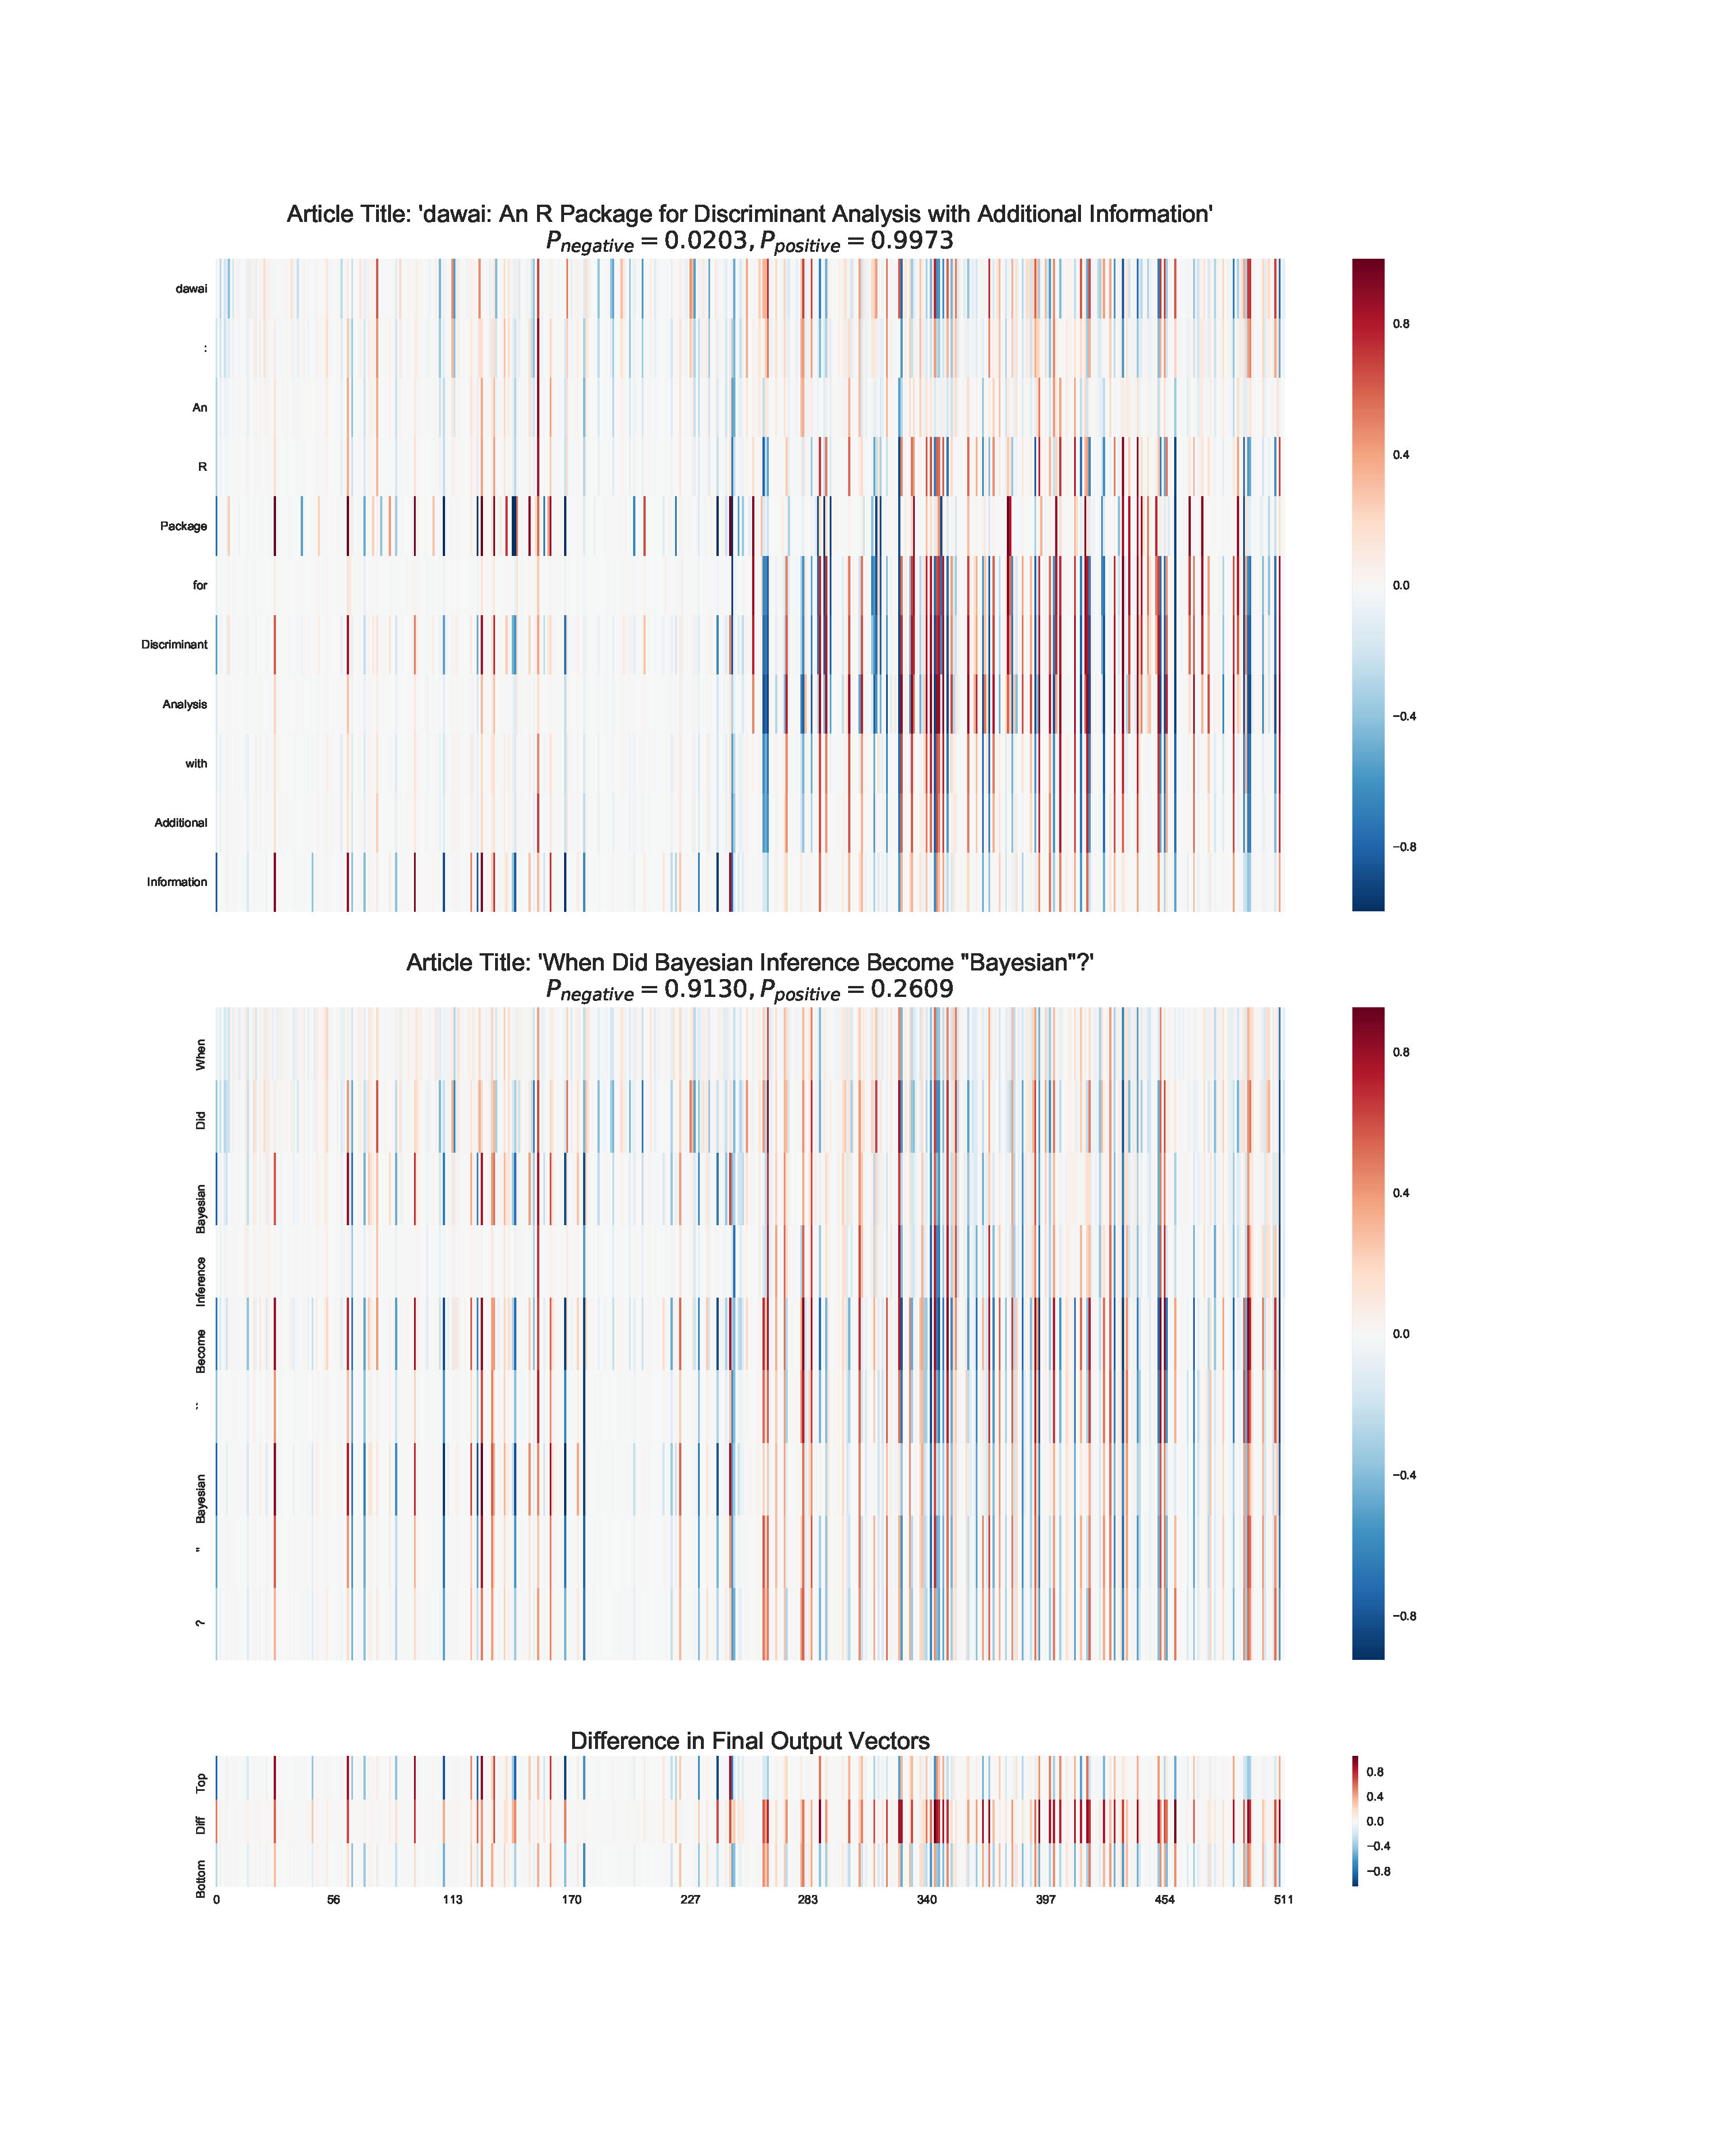
\includegraphics[width=\textwidth]{comparisonTitle.pdf}
	\caption[RNN activations for titles]{RNN activations for each word in two titles; the positive example is on top, the negative below it, and a comparison of each input's final output is shown at the bottom.}\label{title}
\end{figure}

\begin{figure}
	\centering
		\includegraphics[width=\textwidth]{comparisonAbstract.pdf}
	\caption[RNN activations for abstractss]{RNN activations for each word in two abstracts; the positive example is on top, the negative below it, and a comparison of each input's final output is shown at the bottom.}\label{abstract}
\end{figure}

\subsection{Output}

The output from the model is a 2-dimensional vector with the first dimension being the log probability of the input being negative and the second the log probability of it being positive. There is no guarantee that the probabilities sum to 1, but as Figure \ref{pvn} shows the probabilities are mostly symmetric. Thus to get a classification from the model we can simply look at the highest values say that is the classification. When we do this across the entire data set we get the results shown in Table \ref{yt} for each year.

	\begin{table}[H]
	\centering
	\begin{tabular}{|l| cccc|}
		\toprule
		Year& Number of Articles & Not Software &  Software & New Software Percentage\\
		\midrule[2pt]
		2005&	5 235&	4 998&	237&$4.52\%$\\
		2006&	5 806&	5 522&	284&$4.89\%$\\
		2007&	6 255&	5 914&	341&$5.45\%$\\
		2008&	7 085&	6 703&	382	&$5.39\%$\\
		2009&	7 435&	7 047&	388	&$5.21\%$\\
		2010&	7 216&	6 801&	415	&$5.75\%$\\
		2011&	7 767&	7 280&	487	&$6.27\%$\\
		2012&	7 990&	7 519&	471	&$5.89\%$\\
		2013&	8 287&	7 829&	458	&$5.52\%$\\
		2014&	8 336&	7 830&	506	&$6.07\%$\\
		2015&	7 559&	7 095&	464	&$6.13\%$\\
		\midrule[1pt]
		Total & 78 971 &74 538&  4433& $5.61\%$\\
		\bottomrule
	\end{tabular}
	\caption{Per year result across all papers}\label{yt}
\end{table}

Table \ref{jtt} shows the top journals by counts, while Figure \ref{pvy} shows each journal's software and non-software counts. 

\begin{table}[H]
	\centering
	\begin{adjustbox}{center}
	\begin{tabular}{l cc}
		\toprule
		Class & Count & Journal\\
		\midrule
		Highest software count (Training)  &673&	JOURNAL OF STATISTICAL SOFTWARE\\
		& &\\
		Highest software count (Non-training)&171&	\pbox{20cm}{IEEE-ACM TRANSACTIONS ON \\COMPUTATIONAL BIOLOGY\\ AND BIOINFORMATICS}\\
		& &\\ 
		Highest non-software count (Training) & 1 156 & ANNALS OF STATISTICS\\
		Highest non-software count (Non-training) &3 381& STATISTICS \& PROBABILITY LETTERS\\
		\bottomrule
	\end{tabular}
\end{adjustbox}
	\caption{Top journals for each class in training and full dataset}\label{jtt}
\end{table}

\begin{figure}
	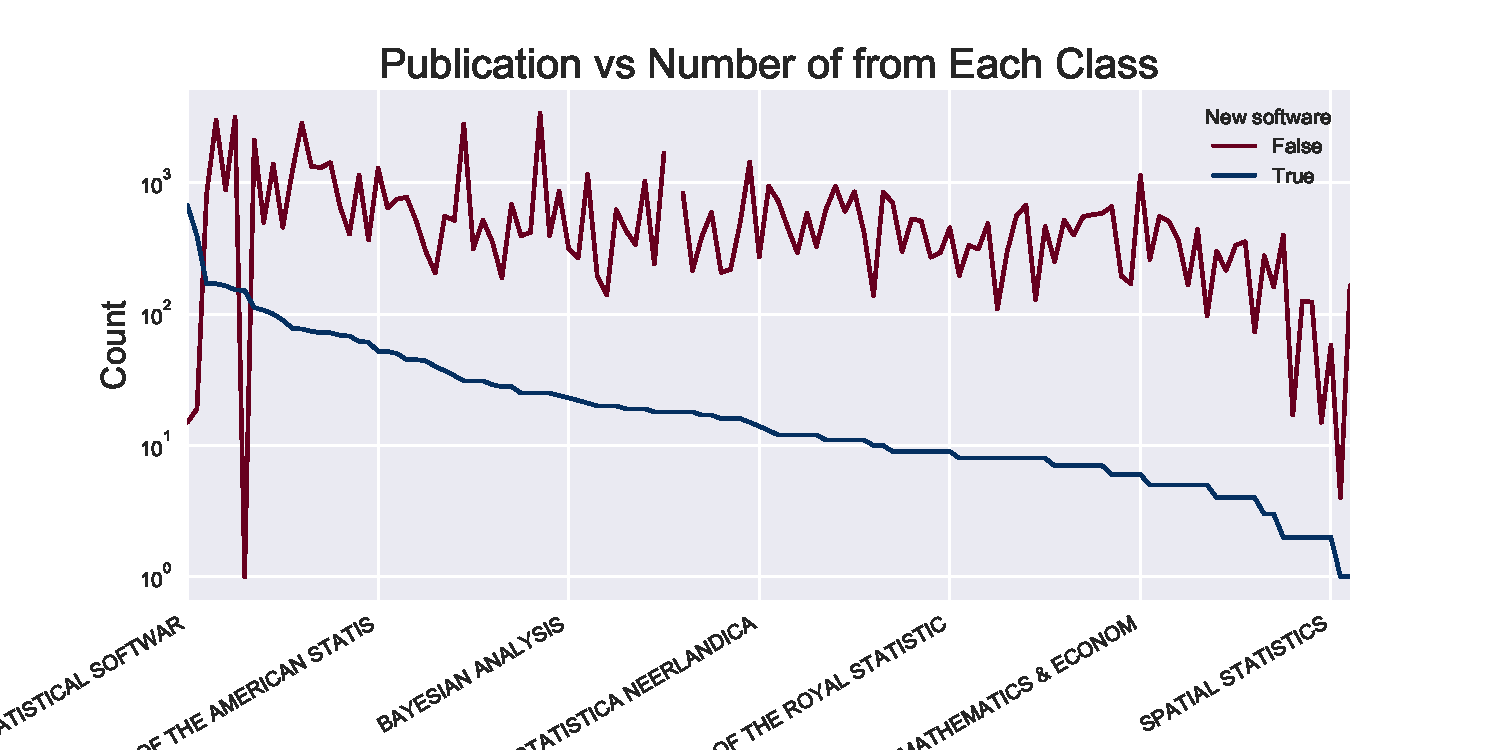
\includegraphics[width=0.9\linewidth]{countvpub.pdf}
	\caption{Counts for each class against each journal, ordered by number of positive examples, note y axis is log}\label{pvy}
\end{figure}

We can also break down the counts per language, as in Table \ref{ptl}. These counts are derived from a very simple sub-string search and as such can not be considered to be very accurate, they are likely under counting most categories. But they do show that the expected result of R being by far the most popular. Interestingly one of the most popular languages JavaScript has no representation.

\begin{table}[H]
	\centering
	\begin{tabular}{lr}
		\toprule
		Language &  count \\
		\midrule
		R           &    566 \\
		Stata       &    130 \\
		Matlab      &     37 \\
		SAS         &     32 \\
		C           &     12 \\
		Mathematica &      7 \\
		Python      &      6 \\
		Java        &      3 \\
		SPSS        &      1 \\
		C++         &      1 \\
		JavaScript & 0\\
		Perl & 0\\
		\bottomrule
	\end{tabular}
	\caption{Per language counts for from positive examples}\label{ptl}
\end{table}
	
\section{Discussion}

As I have shown, the model is capable of identifying complex ideas in textual data. The training set is both relatively small and imperfect; in fact, when the false classifications are examined by an expert, most of them result from errors in the data and not in the model. Thus, by using the model to help generate  cleaner data, a new model could be trained with higher accuracy. The main issue is the false detection rate, which could be reduced by training a cascade of NNs instead of a single one.

These issues aside, the research undertaken herein demonstrates large-scale detection of new software introduced in scientific literature. We can use this data to start making inferences about the usage of software by statisticians. First we can see that a large number of of them likely use a programming language or software tool if $5.6\%$ of all papers are statisticians creating new tools if even five other papers use the tool then $~30\%$ of all papers would have some computational aspect and this is likely greatly understanding the diffusion. We can also see that usage is rising, with 2005 having $1\%$ less usage than 2015, this is likely dues to computational methods becoming more important in the last decade. What is also shown is that computational methods are not clustered in one or two journals, most for most journals there is a $1-4\%$ chance of a random article being a new software tool. This means that most statisticians are reading about computational tools and thus are likely using them. Finally we can see that to no ones surprise R is by far the most dominant language for statisticians.

The next steps are to do biometric and natural language processing on our corpora as there are many questions we can answer. Of interest to us are `\textit{How programming languages distributed across the sciences?}', `\textit{What properties of new scientific software packages cause them to be accepted by a community?}' and `\textit{What is the relationship between success as an article and success as a software tool?}'. All of these questions are important to understanding how software has shaped the way scientists work and how scientists have shaped their tools.

The question most pressing to me is `\textit{What properties of new scientific software packages cause them to be accepted by a community?}' to answer this I would study the activation plots like those in the interpretation section, to find those activations that correspond to the naming of the package and to the naming of the language. These both should exists as they are some of the strongest indicators of a positive sample. From this I can lookup the source code of the package as well as a variety of other pieces of information including if available their entry in repository. This then would let me link WOS ID numbers to software packages at a large scale and from that I can analysis the biometrics of the package. This would let me look for patterns in usage across both the scientific domain and the repository level.


\newpage
\bibliography{Report}{}
%\bibliographystyle{plain}
\bibliographystyle{asr}

\end{document}